% document based on the VU Beta / BSc Thesis template

\documentclass[11pt]{article}
\usepackage{graphicx}
\usepackage{hyperref}
\usepackage[table,xcdraw]{xcolor}

      \textwidth 15cm
      \textheight 22cm
      \parindent 10pt
      \oddsidemargin 0.85cm
      \evensidemargin 0.37cm

%
\usepackage{xcolor}  % Colored text etc.
%
\definecolor{OwnAzure}{HTML}{336699}
\definecolor{OwnCerulean}{HTML}{CAE2FE}
\definecolor{OwnOliveGreen}{HTML}{556B2F}
%
\usepackage[colorinlistoftodos,prependcaption,textsize=tiny]{todonotes}% Add ,disable to the options, to hide the comments
%
%
\usepackage{xargs}                      % Use more than one optional parameter in a new commands
%
\newcommand{\todojacob}[1]{\todo[inline, color=OwnAzure!40]{Jacob: #1}}
\newcommand{\todoalexandru}[1]{\todo[inline, color=orange!40]{Alexandru: #1}}

\newcommand{\thoughts}[1]{\todo[inline, color=OwnOliveGreen!40]{Question: #1}}
\graphicspath{ {./images/} }
\begin{document}

\thispagestyle{empty}
\newcommand{\opendc}{OpenDC}

\begin{center}

Vrije Universiteit Amsterdam

\vspace{1mm}


\includegraphics[height=28mm]{vu-griffioen-white.pdf}

\includegraphics[height=28mm]{atLarge.jpg}

\vspace{1.5cm}

{\Large Bachelor Thesis}

\vspace*{1.5cm}

\rule{.9\linewidth}{.6pt}\\[0.4cm]
{\huge \bfseries LEGO, but with Servers:\par}
{\Large \bfseries Creating the Building Blocks Required to Design Datacenters\par}\vspace{0.4cm}
\rule{.9\linewidth}{.6pt}\\[1.5cm]

\vspace*{2mm}

{\Large
\begin{tabular}{l}
{\bf Author:} ~~Jacob Burley ~~~~ (2599965)
\end{tabular}
}

\vspace*{1.5cm}

\begin{tabular}{ll}
{\it 1st supervisor:}   & ~~dr. Alexandru Iosup \\
{\it 2nd reader:}       & ~~Laurens Versluis
\end{tabular}

\vspace*{2cm}

\textit{A thesis submitted in fulfillment of the requirements for\\ the VU Bachelor of Science degree in Computer Science}

\vspace*{1cm}

\today\\[4cm] % Date

\end{center}

\newpage

\tableofcontents
\newpage
\listoffigures
\listoftables
\newpage


\section*{Abstract}
Will be written last.
\newpage

\section{Introduction} \label{sec:introduction}
	
	\subsection{\opendc{}}
		With the rapid expansion in the use of cloud services by both consumers and businesses \cite{Kushida2015}\cite{mokhtar2013}, the datacenters that house these services must also grow. 
		While many may not ever see the cloud in in terms of its underlying hardware, cloud services are provided by servers, and servers are typically stored in datacenters. 
		The configuration of such servers varies drastically, depending on the intended workload. 
		Relational databases, for example, can have large memory requirements. 
		Likewise, file servers may not need a particularly powerful CPU, but do require a lot of disks, and perhaps even a network card with higher maximum throughput.

		When architecting datacenters, many stakeholders must come together and agree on the various specifications of the data center, each with their own unique set of requirements. 
		System architects will then begin to design a system that meets these requirements. 
		However, such projects also have constraints. 
		Designing a data center is not as easy as buying servers that meet the requirements of the stakeholders and putting them into use. 
		Constraints such as budget or physical space often influence design decisions, with smaller (metropolitan) datacenters with less floor space sometimes making use of higher-density compute nodes, such as blade servers. 
		Designing datacenters is often a complex problem, for which no validated analytical models exist. 
		Despite some academic institutions often being forthcoming with the technologies used in their datacenters, there is no one-size-fits-all approach for data center design, making it hard to determine what hardware you need for a given set of workloads.
		
		We focus in this work on \opendc{}, an open-source Discrete Event Simulator used to simulate the performance of workloads on massive computer systems. 
		Its purpose is to assist in performance testing of datacenters designed by users, with the intention that the information gained can be factored in when these systems are being designed. 
		\opendc{} simulates workloads using traces from the Grid Workload Archive \cite{Iosup2008}, which are provided by participants who contribute to the archive. 
		These traces provide metadata about the scheduling requirements of jobs frequently sent to datacenters, such as CPU usage throughout a job. 
		Using this information in combination with information about the hardware being simulated, \opendc{} can simulate the speed with which a workload will complete, as well as resource usage throughout the workload. 
		These simulations can assist businesses and educational institutions in highlighting and addressing performance concerns in their next-generation environments before any hardware has even been purchased.
	
	\subsection{Problem}
		In its current state, \opendc{} can be used to simulate user-specified workloads on user-designed systems. 
		Users must specify each individual component used, and build out an entire system, effectively doing all of the design work themselves. 
		This requires a high level of technical understanding, and relies solely on the user's knowledge of the intended workload to make component choices. 
		In this way, the reasoning behind component choices has to be expressed by the individual, rather than \opendc{} itself.  

		With the implementation of prefabricated components (\textit{prefabs}), complete collections of components intended for a specific workload can be ``dragged and dropped" into a datacenter design, allowing for accelerated prototyping.
		In this way, hardware choices can be made by \opendc{}, based on which workload(s) the user wants to run.
		As a result, all a user would need to know to begin designing a datacenter would be its intended purpose, and the workloads it would be required to run.
		% A user could then "drag and drop" the components required for certain services into their datacenter design, which would provide at least a starting point to build off of, allowing for accelerated prototyping.

		When working with scalable workloads, prefabs can also provide benefits.
		If the workload relies on homogenous nodes, these nodes can be defined as prefabs, and added into the design as needed for capacity testing.
		Prefabs could consist of a single server, but could also scale up to a rack full of servers, or even a room full of equipment.
		This approach would enable users reliant on homogenous hardware configurations to save their standard configurations as prefabs, further saving time when they need to add more of the same kind of node in new designs.
	
	\subsection{Research Questions}
		In this thesis, we aim to improve the ease of use of \opendc{}, while also implementing a new, easily-expandable representation of datacenter hardware that allows for accurate technical descriptions of hardware. 
		In doing so, we answer the following three questions:
		\todojacob{Reword the RQs to flow a little better and be a little clearer.}
		\begin{itemize}
			\item [\textbf{RQ1:}] How do we design a prefab abstraction that accurately describes important technical and composable features?
			\item [\textbf{RQ2:}] How to further allow operations and extensions of prefabs, and the sharing of data?
			\item [\textbf{RQ1:}] How can we test and validate the use of prefabs to define hyperconverged/HPC datacenter topologies?
		\end{itemize}
	
	\subsection{Approach}
		The approach begins with understanding the shortcomings of the current implementation of topologies in \opendc{}.
		Next, we seek to understand the components that are important to represent in the datastructure, as well as identify components we no longer need to represent.
		From here, we examine a variety of common methods of representing data, and assess their suitability towards our desired way of representing datacenter hardware.
		Following on from this, we present a datastructure design, as well as the decisions made during the design process, and validate it through a prototyping stage.
		We also assess what interactions need to be supported on the datastructure, and ensure that the datastructure design supports these interactions.
		Lastly, we implement the datastructure design and accompanying technologies into \opendc{}.
	
	\subsection{Main Contribution of the Work}
		This thesis pioneers a new approach to representing datacenter hardware within a datacenter simulator.
		The main contributions of this thesis are:
		\begin{enumerate}
			\item A design for a datastructure that can be used to store datacenter hardware representations that is also easily usable and expandable, as well as an evaluation of said design in terms of the suitability of the datastructure for purpose.
			\item An implementation of this design into the main codebase of \opendc{}, as well as an evaluation of this design comparing usability to the previous version of \opendc{}.
			\item An example library of components intended for High Performance Computing for use within \opendc{}, built using the design specified in this thesis.
		\end{enumerate}
	
	\subsection{Thesis Outline}
		The first chapter provides a short introduction to the current state of datacenter design, as well as the current state of OpenDC. 
		Chapter 2 provides more background on how modularity is currently used in computing, both in datacenters and in fields such as software engineering. 
		In Chapters 3 and 4, we design a prefab datastructure, reason about the choices that have been made during the design process, and touch on the process of implementing our chosen datastructure into the \opendc{} codebase.
		Chapter 5 provides an assessment of the suitability of the datastructure and technologies we chose, now that they have been implemented in \opendc{}.
		Finally, we discuss both the conclusion and future of this endeavour in Chapter 6.
	

	

\newpage

\section{Background} \label{sec:background}
	Servers today are used for a wide variety of things, ranging from hosting video games all the way up to calculations for nuclear research at the European Organization for Nuclear Research (CERN) \cite{Andrade2012}.
	As the need for servers grows, in part due to a massive increase in the demand for cloud services \cite{Pring2009}, the size of datacenters will also have to grow.
	As a result, datacenter operators will have design and organise these new datacenters into a logical organisational structure.
	\subsection{A Topological View of Datacenters}
		\begin{figure}[ht!]
			\centering
			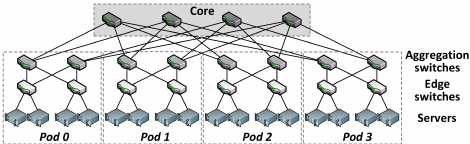
\includegraphics[width=8cm]{couto2012/Fat-tree-with-4-port-switches-n-4.png}
			\caption[A conventional network-focused datacenter topology]{A conventional network-focused datacenter topology \cite{Couto2012}}
			\label{fig:networktopology}
		\end{figure}
		In general, individuals working with datacenters think about their datacenter in terms of its topology. 
		Often, this takes the form of a network topology \cite{Couto2012}, where a spanning tree is built from all of the participating nodes. 
		For \opendc{}, however, it is important to consider the parent-child relationships between the hardware components themselves. 
		For example, we can consider a chassis residing within a given rack to be a child of that rack, with good datacenter practice requiring that an in-use chassis is not kept outside of a rack.
		By defining these inter-component relationships, we can build our own spanning tree model, which allows us to easily manipulate parent objects and all of their children by simply moving the parent object elsewhere in the tree, reshaping our topology.
		\begin{figure}[ht!]
			\centering
			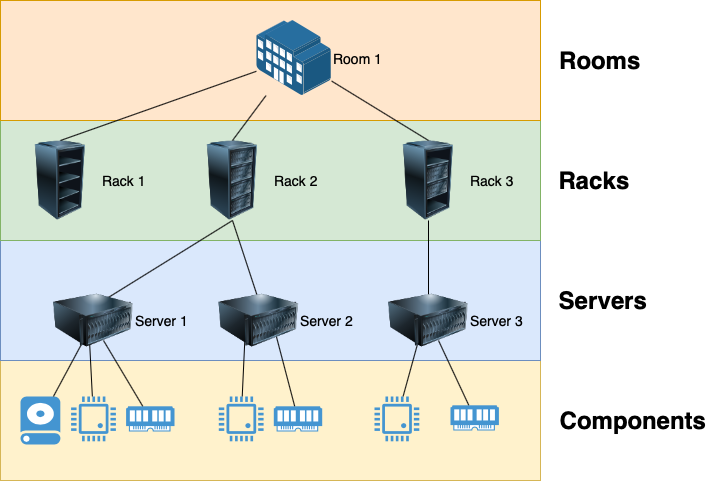
\includegraphics[width=8cm]{opendc-topology.png}
			\caption[A simple topology in OpenDC]{A simple topology in OpenDC}
			\label{fig:example-opendc-topology}
		\end{figure}
		\thoughts{I've chosen to not include details such as racks being children to tiles in this figure, because a) its quite early in the thesis and b) I don't think including details such as tiles is particularly relevant for the comparison (or for prefabs themselves). What do you think?}

	
	\subsection{Modularity in Computing}
		In software architecture, it is becoming increasingly common to rely on frameworks and libraries written by others in the software engineering community. 

		This process would be akin to the modularity already seen in software engineering, where a programmer may import a library (often written by someone else) to enable certain functionality in their program. 
		The programmer often only uses one or two functions from this library, and does not necessarily understand how these functions work (nor do they need to).
		It is usually not necessary to understand the full workings of such a library, as the benefit comes from its utility in meeting certain requirements. 
		We can view these software modules as prefabricated software, which an individual may add into their project with ease. 
		Such a module may be added manually, by copying the relevant source files into the project, or may be added by means of a package manager.
		
		\verb|npm| is a package manager for \verb|node.js| that seeks to make installing dependencies much easier for developers \cite{Wittern2016}.
		For open-source projects a developer can include a file listing all of the external packages they used in their project, as well as the specific versions of each of these packages, so that another individual can easily run the authors software on their own machine.
		\verb|npm| also enables package authors to publish their packages in an online registry, so that other developers may download and use them.
		It follows, then, that it would be helpful to be able to describe datacenter hardware, and share these descriptions, in a similiar way. 

		With the advent of PaaS and particularly SaaS offerings from major cloud providers, developers can implement entire layers of their software stack with just a few clicks. 
		These layers still run in virtual machines, but the developer does not need to concern themselves too much with building or maintain the hardware or operating system.
		This concept is already offered by some cloud providers: DigitalOcean is a Virtual Private Server (VPS) provider that harnesses a ``marketplace" of pre-configured VPS templates (known as ``1-Click Apps") in order to simplify use of the platform \cite{DigitalOcean2020}. 
		Customers can then easily add a pre-configured VPS to their environment, without having to worry about operating system installation, configuration, or maintenance. 
		Templates provided through the platform are typically created by the vendors of the software used in each template, and are thus of high quality and suitability for the chosen application.

		In the realm of hardware, we are also seeing modularity emerge. 
		Hewlett Packard Enterprise (HPE) produces a scalable server design, whereby more compute (in terms of CPU, Graphics and Memory) can simply be added as necessary \cite{Bang2020}.
		A single operating system instance runs on this hardware, which can (at the time of writing) be expanded with up to 32 sockets, each with up to 28 physical cores per socket.
		It is thus possible to begin with a single system, and simply add ``more of the same" when expanding datacenter capacity.

		At a more macro level, Schneider Electric provide prefabricated, modular structures to house, power, and cool datacenters \cite{Torell2014, Torell2017}.
		While the offering from Schneider Electric does not include recommendations for actual compute hardware, IBM offers the possibility of a completely modular datacenter \cite{IBM2014}.
		Such a datacenter can quickly be scaled up or down depending on the needs of the customer, using pre-designed components for power, cooling, and floorspace. 
		These prefab datacenters are real-life examples of how datacenter design can be modular.

	
	\subsection{Formats for Specifying Datacenter Topology Modules}
		When considering a new format for representing our new datastructure, we must first identify the important qualities that a suitable format must have. 
		A functional requirement for the format is that it must support nested objects. 

		The database used in version 1.x of \opendc{} contains 35 SQL tables, 20 of which are used to store topologies.
		As a result, adding hardware items to the database requires a complex set of queries, with deletions and modifications requiring additional queries.
		In order to reduce the complexity associated with \opendc{}, we seek a storage format that allows us to store entire prefabs (as well as topologies) within a single object.
		The advantage of such an approach is that the database then only has to support the adding, updating and deleting of prefabs and other topology objects.

		We consider several formats for representing our datastructure.
		\todojacob{Rewrite in progress}
		First, we consider \textit{YAML Ain't Markup Language} (YAML) \footnote{\url{https://yaml.org/spec/1.2/spec.html}} as our document format.
		YAML is both human as well as machine readable, and supports nested object hierarchies.
		However, we find that YAML is not suitably human-readable.
		It relies on indentation for distinguishing levels of hierarchy, with no clear boundaries delimiting separate objects.

		\textit{Extensible Markup Language} (XML) \footnote{\url{http://www.w3.org/TR/REC-xml}} is a common language for storing and representing documents that is used in many web applications.
		It is both human and machine readable by design, and is well suited to nested object hierarchies, making it a strong contender to be used to store prefabs.
		However, XML requires parsing.
		The current \opendc{} frontend is written in \verb|ReactJS|, which does not natively support parsing XML without the use of an external library.
		As we prefer not to add additional dependencies to \opendc{}, we do not find XML to be a suitable choice as a document format.
	
	\subsection{Domain-Specific Modules}
		Datacenters have many intended uses, depending on the intended domain of the datacenter, such as High Performance Computing (HPC), scientific computing, business-critical applications, generalized cloud infrastructure, etc.
		The design of datacenters, as well as the component choices made during the design process, varies significantly depending on the domain it is used in.
		Some datacenter owners within the field of HPC may choose to focus on a hyperconverged infrastructure, where a many-core approach is taken to provide massive performance density.
		This allows for high performance, even within small metropolitan datacenters such as ones commonly found at universities, where space comes at a premium.

		In a business-critical environment, hardware may be physically replicated across both racks and physical locations, so that even a total datacenter loss would have a reduced impact on business operations.
		In such a scenario, hardware is not chosen based on the suitability for one application, but to support the flexibility to be able to run any application in virtual machines.
		This is especially common in this field, with the intention of further reducing downtime.
		Virtual machines can be migrated between physical hosts while still running when hardware maintenance is required.
		It is also possible to add resources to a virtual machine without power loss, dynamically scaling them to jobs.

		Conversely, other datacenter owners may focus on scientific computing \cite{SURF2020}.
		\todojacob{More scientific computing references}
		These datacenters are designed differently, with a high number of nodes running a baremetal operating system.
		The configuration of these nodes varies, depending on the intended use of the node.
		Nodes are then categorized into performance tiers based on their intended use.
		Performance tiers are then chosen by customers depending on the kind of workload they want to run - for example, GPUs may be installed in the nodes in tiers intended for Machine Learning workloads.

		Prefabs specific to certain domains can be represented in \opendc{}, with different performance tiers included within each domain.
		In this way, users can easily build massive, homogenous systems by selecting the node specific to their performance target, and using it as a starting point.

\newpage

\section{A Design for a Representation of Data Center Hardware} \label{sec:design}
	Servers within a datacenter are typically feature rich, with certain features included to differentiate them from their competitor.
	There are characteristics of the hardware (such as chassis colour) that have little relevance when designing a datacenter.
	Conversely, properties of the hardware such as the power draw, or the heat output, are important with regards to the planning of the datacenter infrastructure, as there will be a performance impact if these properties are not accounted for.
	When representing datacenter hardware in a datastructure, it is important to consider which aspects of the hardware are relevant to represent.
	
	\subsection{The Goal of Prefabs: Requirements Analysis}
		When designing our new datastructure, it is important to consider the potential use-cases for key stakeholders.
		We identify our stakeholders to be researchers in the fields of distributed or large-scale computer systems, students in the same field, and datacenter operators in both industrial and academic settings.

		Both researchers and students would benefit from the addition of prefabs to \opendc{} in the same way that developers (and other customers) benefit from modern PaaS offerings, only having to focus on which services they want to run in their datacenter.
		Additionally, datacenter operators using \opendc{} for datacenter design and testing may also see a benefit from prefabs. 
		Cloud service providers who provide IaaS services typically use homogenous hardware configurations, with different configurations for each performance tier. 
		With prefabs, it would be straightforward to create a prefab that is representative of a given performance tier, and then clone it when performing capacity planning during periods of growth.
		Lastly, given the widespread support for the sharing of information within academia, the ability to share prefabs would be an important addition to the features of \opendc{}.

		From these use-cases, we can already define some functional requirements for prefabs.
		\begin{itemize}
			\item [\textbf{FR1:}] Users should be able to use existing topology definitions as a basis for new prefabs.
			\item [\textbf{FR2:}] Users should be able to add prefabs into existing topologies, using them as building blocks to enable faster prototyping and design.
			\item [\textbf{FR3:}] Users should be able to determine what tasks a given prefab is suited for, by means of a labelling mechanism. Prefabs could then be labelled to indicate, for example, that they are intended for highly parallelizable workloads.
			\item [\textbf{FR4:}] Users should be able to easily share their prefab designs with others.
			\item [\textbf{FR5:}] \opendc{} should provide some example prefabs based on servers that are popular in the market. These prefabs would provide a building block for users to get started with.
		\end{itemize}

	\thoughts{This needs to feel a little more fluid}

	\subsection{A Model for Datacenter Representation}
		In this research, we provide a model for representing datacenter hardware. 
		This model is not the first of its kind: Andreadis et al created a model for datacenter hardware in order to model scheduling in \opendc{} \cite{Andreadis2018}. 
		Our model, however, offers more detail, storing more characteristics of the hardware within.
		When designing the model, it is important to consider that a large part of its purpose is to increase usability of \opendc{}. 
		As a result, we choose to represent lots of hardware characteristics that are not used by the simulator, but provide useful information to the user. 
		Brands of hardware are not necessary in order to simulate workloads, but they are useful when a user is making design decisions, or presenting their design to a wider audience.
		Conversely, performance metrics such as how many millions of instructions per second (MIPS) a processor can execute are of utmost importance to the simulator when extrapolating performance numbers, but are generally meaningless to stakeholders without a technology background.
	
	\subsection{A Definition and Design of a Datastructure for Storing Prefabs}
		In order to store our datacenter hardware representation within \opendc{}, we define a datastructure to represent the datacenter hardware. 
		This datastructure aims to be simple to understand, as well as easily expandable in order to represent hardware configurations that we do not focus on in this research (i.e. blade servers, or other chassis that may contain multiple/unconventional motherboards). 
		For this reason, we choose to use JavaScript Object Notation (JSON) \footnote{\url{https://www.json.org/json-en.html}} to store our datastructure. 
		This supports our goals of ease of use and expandibility, as JSON is a human-readable industry-standard object storage format that can be extended to represent a variety of objects.

		In order to further the goal of simplifying working with \opendc{}, we also transition the storage database away from SQL, towards a NoSQL design.
		We choose MongoDB as a document storage solution due to its ease of use, as well as its flexibility.
		MongoDB supports the insertion of JavaScript Object Notation (JSON) objects.
		JSON is an expressive, industry-standard object storage format that is widely used in web-based applications.
		It is both human-readable, and supports nested object hierarchies.
		The support for nested objects is crucial to us in order to achieve some of our functional requirements, namedly \textbf{FR1} and \textbf{FR2}, as it allows for easier insertion into the object.

		The author of this thesis was involved in the transition from SQL to noSQL, which involved the porting of the current database schema to MongoDB. 
		This effort also involved porting the existing \opendc{} API from Python 2.7 to Python 3, and rewriting the API to include new endpoints for prefabs, as well as the new topology structure.


	\subsection{Designing Ways to Create and Interact with Prefabs}
		When determining interactions we prefabs, we must define a set of operations that meets the functional requirements defined earlier.
		

\newpage

\section{Implementation of a Prototype} \label{sec:implementation}
	In this section, we describe the prototyping stage of this project.
	We cover the motivations behind prototyping, as well as the processes of designing, implementing and testing the prototype.
	\subsection{Why Prototype?}
		Prototyping is an important part of our design process for implementing the new topologies in \opendc{}.
		The design proposal requires the implementation of certain new technologies (such as MongoDB) which we are unfamiliar with.
		As a result, prototyping provides us with a way of becoming familiar with these new technologies, as well as assessing their suitability, before we begin the process of implementing them into the existing \opendc{} codebase.
		We also can create prototypes of the datastructure, as well as the corresponding interactions with it, and assess the suitability of the datastructure with regards to the interactions we require it to perform.
	
	\subsection{Creating a Prototype}
		The two main learning outcomes of prototyping are to explore how we can best implement and interact with MongoDB, and to iteratively improve our datastructure design.
		As a result, the prototype consists of three components: a MongoDB instance, a Python module that interfaced with the database, and a second Python application to serve as a rudimentary frontend. 
		This configuration has been chosen to be relatively close to how \opendc{} already implements its database connections, which also uses a Python module to abstract away most database interactions.

		MongoDB has been chosen in order to easily facilitate the storage of our JSON objects.
		MongoDB stores documents in a JSON-like format internally, and has strong library support for inserting, modifying and exporting said documents, making it relatively straightforward to re-implement our database connection.
		\todojacob{more on this}

	\subsection{Validating Prototypes}
		In order to validate our prototype, we need to determine...
		\thoughts{KLM testing on prototype}

	\subsection{Lessons Learned}
		During prototyping, we learnt many things that influenced the decisions we made during the implementation phase.

		Firstly, we opted not to enforce schema validation on the collections within our database.
		The reasoning behind this decision was that schema validation in the database added unnecessary complexity, and limited the shape of our data (and thus hardware that could be represented).
		We instead choose to check for required fields (such as the topology name, or the prefab visibility) within the API.
		This allows for topologies to contain hardware configurations that may not have been considered during the design process, while also allowing us to make assumptions about certain aspects of the datastructure.

		We also became more familiar with certain aspects of MongoDB, including the differences between Binary JSON (BSON) and JSON.
		When we began working with MongoDB, we operated under the assumption that MongoDB would export objects in JSON, just as it can be given JSON objects to import.
		However, this assumption turned out to be incorrect. 
		During testing of topology import functionality, we attempted to import a topology that we had exported to JSON.
		When this test failed, we discovered that MongoDB does not use pure JSON for exports.
		Instead, it exports objects in BSON, the same format it uses to store objects internally within the database.
		MongoDB simply stores files in a binary format internally, and converts them back to something human-readable when you export them. 
		However, the human-readable format that MongoDB uses is not JSON, but is deceptively similiar: BSON uses single quotes (') where JSON uses double quotes(").
		As a result, we implemented a conversion from BSON to JSON within our API, so API responses are formatted in proper JSON that can be used by the frontend.

		We also learnt a lot about the differences between MongoDB and SQL, which allowed us to improve how we implement this new database technology throughout \opendc{}.
		We moved from a database structure consisting of many tables, to one with very few.


\newpage

\section{Domain-Specific Prefabs in \opendc{}}
	In this section, we explore the High Performance Computing domain, and validate our prefab representation by creating prefabs for some common servers used within this domain. of some of the HPC-oriented server offerings from the top 3 OEMs by market share in Q1 2020.
	
	\subsection{Representing Domain-Specific Hardware with Prefabs}
		In order to select server SKUs to represent, we identified the top server OEMs by market share in Q1 of 2020 \cite{Macatee2020}. These summarised findings are presented in Table 1.
		\begin{table}[]
		\centering
		\begin{tabular}{|l|ll|ll}
		\cline{1-3}
		Company                                             & Units Shipped                   & Market Share                     \\ \hline
		\cellcolor[HTML]{9AFF99}Dell Technologies           & \cellcolor[HTML]{9AFF99}474,011 & \cellcolor[HTML]{9AFF99}18.4\%   \\
		\cellcolor[HTML]{9AFF99}HPE/New H3C Group           & \cellcolor[HTML]{9AFF99}377,544 & \cellcolor[HTML]{9AFF99}14.7\%   \\
		\cellcolor[HTML]{9AFF99}Inspur/Inspur Power Systems & \cellcolor[HTML]{9AFF99}211,007 & \cellcolor[HTML]{9AFF99}8.2\%    \\
		Lenovo                                              & 153,570                         & 6.0\%                            \\
		Super Micro                                         & 132,001                         & 5.1\%                            \\
		Original Design Manufacturer Direct sales                                         & 770,446                         & 29.9\%                           \\
		Rest of Market                                      & 456,841                         & 17.7\%                           \\ \cline{1-3}
		\textbf{Total}                                      & \textbf{2,575,439}              & \textbf{100.0\%}                 \\ \cline{1-3}
		\end{tabular}
		\caption{Market Share Distribution amongst Server OEMS in Q1 of 2020}
		\label{table:1}
		\end{table}
		We chose the individual manufacturers with the top 3 market shares (highlighed in green) as our target manufacturers.
		We then chose the HPC-oriented server offerings from each of these manufacturers, and attempted to model them in the prefab datastructure.
		The server selection process varied slightly by manufacturer, but generally, we sought out servers that the manufacturer described to be suited for HPC, or other intensive compute workloads.
		For each server, we then attempted to represented it with as powerful of a configuration as possible, populating all sockets, DIMM slots and storage bays.
		For HPE's Superdome Flex, we also included the optional GPUs in the configuration.
		Other configurations supported GPUs, but as they were not included in any of the available OEM configurations, we opted not to include them in these configurations.

	\subsection{Accuracy of Hardware Representation}
		Ultimately, we find the accuracy of our hardware representations to be sufficient.
		There are aspects of each server that are not represented in our prefabs, such as the presence of Out-of-Band management, or network cards.
		These components currently do not form part of our topology design, as they are currently not relevant to our simulations.

		Additionally, there are aspects of hardware that we have chosen not to represent in this thesis, such as multi-node chassis.
		As a result, it was not possible to model hardware such as HPE's ``Apollo" line of high-density HPC servers, or Dell's PowerEdge Blade Enclosure.
		Such hardware is seen frequently in the HPC domain, providing high levels of compute density, further solidifying the notion that \opendc{} should support these kinds of representations in the future.
		However, it is still possible to simulate performance aspects of these multi-node systems, as they can be represented within \opendc{} as individidual servers.
		As a result, this limitation only impacts physical datacenter design.

		Lastly, the ``Inspur Power Systems FP5180G2" prefab contains IBM POWER9 processors, based on the Power Instruction Set Architecture \cite{IBM2017}.
		These CPUs exhibit different performance characteristics than Intel or AMD processors, in part due to different instructions exposed by the CPU.
		This difference is not accounted for by the simulator in \opendc{}, and there is currently not a provision for representing this difference in our topology structure.
		Again, this is an improvement that could be made in the future, and would be relatively straightforward to represent given the flexible nature of our topology structure.


	\subsection{Applying this Approach to Other Domains}
		We find that this approach would be straightforward to apply to other domains.
		Most manufacturers provide information about intended workloads for their hardware offerings, allowing for relatively straightforward server selection.
		For smaller domains (such as game streaming), however, it may be beneficial to consider the performance requirements of the domain with regards to speciality hardware, as these domains are not always as clearly differentiated.

\newpage

\section{Evaluation of Design \& Implementation} \label{sec:evaluation}

\newpage

\section{Conclusion} \label{sec:conclusion}
	\subsection{Summary}
	
	\subsection{Future Work} \label{sec:future-work}
	\todojacob{Adding this here for now, will likely merge future work into conclusion at a later date.}
	Looking forward, there are several areas of interest that it would be beneficial to visit in future research.

	Firstly, there are many more characteristics of datacenter hardware that we could extend \opendc{} to represent. 
	We currently do not focus on high-density servers with multiple mainboards (such as blade servers) in each chassis in this thesis. 
	We could also extend rack prefabs to include networking hardware required for the topology. 
	The addition of networking hardware would also be beneficial for modelling Storage Area Networks (SANs) as well as topologies that include nodes comprised of multiple units, such as HP's Superdome Flex concept\footnote{\url{http://hpe.com/superdome}}.
	Hardware for managing the power distribution throughout a topology would also be an important future expansion.
	Uninterruptible Power Supplies (UPSes) and Power Distribution Units (PDUs) are critical to the health of datacenter hardware, and take up rackspace.
	As a result, it would be useful to represent this hardware in \opendc{} in the future, as per-rack power limits would be dictated by the presence of such hardware.

	Next, the \opendc{} user interface could be further refined, to increase functionality and improve usability.
	A possible addition to the UI could be a powerful text-based console within the browser, so that the creation and manipulation of topologies and prefabs could become even more intuitive, allowing for even faster (and reproducible) prototyping.
	While the features we have introduced in this thesis are aimed towards a more general, less technically-oriented audience, the above feature would be aimed at users with more experience in datacenter design.

	Additionally, we could extend domain-specific prefabs to include more domains.
	So far, we have covered the domain of High Performance Computing, but there are many more that remain that are extremely relevant to the direction of the industry.
	Areas such as cloud gaming, or business-critical infrastructure have different requirements of their hardware choices, and so their topologies and thus their prefabs would likely look quite different from what we have explored so far in this thesis.
	Future work could investigate what kinds of hardware is used in these fields, and what useful prefabs would look like in these domains.

	Lastly, it would be interesting to design a means for \opendc{} to simulate user-specified workloads on systems designed by \opendc{} itself. 
	\opendc{} would be able to leverage a large database of performance data to make component choices based on the workload specified by the user. 
	\opendc{} could even be taught how to perform such a task, using Machine Learning with existing datacenter designs as training models.
	Research could be carried out to determine which hardware characteristics translate best into high performance for certain workloads, leading to objectively performant prefabs designed for those workloads.
	These research-based prefabs would then serve to validate the prefabs that \opendc{} learns to build, and further help develop this functionality.
	In this way, the system would be designed for the best objective performance at the specified workload, potentially adherent to specified constraints such as financial or power budget.
	If desired, the level of user interaction could be minimal to none, perhaps only requiring small changes to the design.







\newpage
% For more on bibliography styles, see 
% https://www.overleaf.com/learn/latex/Bibtex_bibliography_styles
\bibliographystyle{abbrv}
\bibliography{main}


\end{document}
% \end{document}



